\documentclass[journal,twoside,web]{ieeecolor}
\usepackage{generic}
\usepackage{cite}
\usepackage{amsmath,amssymb,amsfonts}
\usepackage{algorithmic}
\usepackage{graphicx}
\usepackage{algorithm,algorithmic}
\usepackage{hyperref}
\hypersetup{hidelinks=true}
\usepackage{textcomp}
\usepackage{multirow}
\def\BibTeX{{\rm B\kern-.05em{\sc i\kern-.025em b}\kern-.08em
    T\kern-.1667em\lower.7ex\hbox{E}\kern-.125emX}}
\markboth{\hskip25pc IEEE JOURNAL OF BIOMEDICAL AND HEALTH INFORMATICS}
{Martínez-Corral \MakeLowercase{\textit{et al.}}: Sistema de Inferencia Difusa para Clasificación de Comportamiento Sedentario}
\begin{document}
\title{Un Sistema de Inferencia Difusa para la Clasificación Interpretable del Comportamiento Sedentario mediante Dispositivos Wearables: Un Estudio de Validación Longitudinal con Validación Cruzada Leave-One-User-Out}

\author{Luis A. Martínez-Corral$^{1}$, 
David R. López-Flores$^{2}$, 
Javier Camarillo-Cisneros$^{3}$, 
Celia María Quiñonez-Flores$^{4}$, 
and Abimael Guzmán-Pando$^{1,*}$
\thanks{Manuscrito recibido [Fecha]; revisado [Fecha]; aceptado [Fecha]. Fecha de publicación [Fecha]; fecha de versión actual [Fecha]. Este trabajo fue apoyado en parte por [Agencia de Financiamiento] bajo el Grant [Número]. (Autor correspondiente: Abimael Guzmán-Pando.)}
\thanks{$^{1}$Luis A. Martínez-Corral y Abimael Guzmán-Pando están con el Laboratorio de Investigación en Inteligencia Artificial y Computación Médica (LIIACOM), Facultad de Medicina y Ciencias Biomédicas, Universidad Autónoma de Chihuahua, Chihuahua 31125, México (e-mail: lmartinez@uach.mx; aguzmanp@uach.mx).}
\thanks{$^{2}$David R. López-Flores está con el Tecnológico Nacional de México, Instituto Tecnológico de Chihuahua, Chihuahua 31200, México (e-mail: david.lf@chihuahua.tecnm.mx).}
\thanks{$^{3}$Javier Camarillo-Cisneros está con el Laboratorio de Química Física Computacional, Facultad de Medicina y Ciencias Biomédicas, Universidad Autónoma de Chihuahua, Chihuahua 31125, México (e-mail: jcamarillo@uach.mx).}
\thanks{$^{4}$Celia María Quiñonez-Flores está con la Facultad de Medicina y Ciencias Biomédicas, Universidad Autónoma de Chihuahua, Campus II, Chihuahua 31125, México (e-mail: cquinonez@uach.mx).}
\thanks{ORCIDs: L.A. Martínez-Corral: 0009-0002-9635-0330; D.R. López-Flores: 0000-0003-4016-0845; J. Camarillo-Cisneros: 0000-0001-7878-1546; C.M. Quiñonez-Flores: 0000-0003-0740-5783; A. Guzmán-Pando: 0000-0003-0819-0438.}}

\maketitle

\begin{abstract}
El comportamiento sedentario (CS) constituye un factor de riesgo independiente para enfermedades crónicas no transmisibles, requiriendo herramientas objetivas e interpretables para su monitoreo continuo. Este estudio desarrolla y valida un Sistema de Inferencia Difusa Mamdani interpretable para clasificar patrones semanales de sedentarismo utilizando datos longitudinales de Apple Watch (N=10 usuarios, 1,337 semanas-observación). Ante el fracaso de enfoques supervisados tradicionales (Redes Neuronales Artificiales con R²<0 debido a N pequeño y ausencia de relación biométricos-calidad de vida), implementamos una estrategia dual data-driven: (1) clustering no supervisado K-Means (K=2, Silhouette=0.232) como Verdad Operativa (GO), y (2) sistema difuso con 4 variables de entrada normalizadas antropométricamente (actividad relativa, superávit calórico basal, HRV-SDNN, delta cardíaco) y 5 reglas expertas basadas en conocimiento fisiológico. La validación mediante concordancia difuso-clustering alcanzó F1-Score=0.840 (Recall=0.976, Precision=0.737, MCC=0.294). La validación cruzada Leave-One-User-Out (LOUO) demostró generalización inter-usuario robusta (F1=0.847±0.041, CV=4.8\%), superior a splits train/test tradicionales que presentan fuga temporal. El análisis de robustez reveló contribución sinérgica crítica de variables cardiovasculares: el modelo reducido (2V) colapsó 50\% en rendimiento vs modelo completo (4V), demostrando que HRV-SDNN, débil predictor univariado (p=0.562), resulta esencial en contexto multivariado no-lineal. Este pipeline metodológico proporciona una plantilla reproducible para análisis riguroso de datos longitudinales wearables en estudios piloto con N<30, priorizando interpretabilidad clínica sobre precisión de caja negra.
\end{abstract}

\begin{IEEEkeywords}
Comportamiento sedentario, dispositivos wearables, Apple Watch, lógica difusa, sistema de inferencia Mamdani, clustering K-Means, validación cruzada LOUO, inteligencia artificial interpretable, salud digital, biomarcadores digitales, ingeniería de características, imputación jerárquica.
\end{IEEEkeywords}

\section{Introducción}
\label{sec:introduccion}

\IEEEPARstart{E}{l} comportamiento sedentario, definido operacionalmente como cualquier actividad en vigilia caracterizada por un gasto energético inferior o igual a 1.5 equivalentes metabólicos (METs) en postura sentada, reclinada o acostada, ha emergido como un determinante de salud pública independiente del nivel de actividad física moderada-vigorosa \cite{Bull2020,WHO2020}. Meta-análisis recientes basados en estudios prospectivos con más de 1 millón de participantes confirman que el tiempo sedentario prolongado se asocia con incrementos del 20-30\% en el riesgo de mortalidad por todas las causas, diabetes mellitus tipo 2 y enfermedad cardiovascular, incluso en individuos que cumplen las recomendaciones mínimas de 150 minutos semanales de actividad moderada \cite{Guthold2020}. La prevalencia global de inactividad física supera el 27.5\%, con tendencias ascendentes proyectadas para alcanzar el 35\% en 2030 si no se implementan intervenciones efectivas, generando una carga económica estimada en 67.5 billones de dólares anuales en costos sanitarios directos e indirectos. En este contexto, la Organización Mundial de la Salud identifica la medición objetiva y el monitoreo continuo del sedentarismo como prioridad estratégica para la próxima década, enfatizando la necesidad de desarrollar tecnologías escalables, costo-efectivas y culturalmente adaptables que permitan la vigilancia epidemiológica en tiempo real y la personalización de intervenciones conductuales basadas en datos de vida libre.

La medición objetiva del CS mediante acelerometría triaxial integrada en dispositivos wearables de consumo masivo (e.g., Apple Watch, Fitbit, Garmin) ha revolucionado la epidemiología del comportamiento durante la última década \cite{Henriksen2018,Doherty2021}. Estos dispositivos permiten cuantificar patrones de actividad física en condiciones de ``vida libre'' (free-living) con alta resolución temporal ($\geq$ 1 Hz) y durante períodos extensos (semanas a años), eliminando el sesgo de recuerdo y deseabilidad social inherente a cuestionarios de auto-reporte como el IPAQ o GPAQ \cite{White2019,Strain2020}. Sin embargo, la transformación de señales biométricas crudas (aceleración, frecuencia cardíaca, fotopletismografía) en clasificaciones clínicamente interpretables de sedentarismo presenta desafíos metodológicos no triviales.

\subsection{Desafíos en Clasificación Automática de Comportamiento Sedentario}

Los enfoques actuales de clasificación automática de CS basados en aprendizaje automático enfrentan tres limitaciones críticas que restringen su adopción clínica a gran escala:

\textbf{1) Problema de Interpretabilidad.} La mayoría de algoritmos de alto rendimiento emplean modelos de ``caja negra'' (deep neural networks, random forests, gradient boosting) cuyas decisiones son opacas para profesionales de la salud \cite{Rajkomar2019,Molnar2020}. Esta falta de transparencia genera desconfianza clínica y dificulta la auditoría de errores, especialmente crítica en contextos de salud donde decisiones algorítmicas pueden impactar intervenciones terapéuticas. El movimiento reciente hacia ``IA Explicable'' (XAI) en salud digital \cite{Escalante2023} ha evidenciado que la interpretabilidad no es un lujo académico sino un requisito ético y regulatorio.

\textbf{2) Dependencia de Tamaños Muestrales Grandes.} Los enfoques supervisados tradicionales requieren conjuntos de datos etiquetados con cientos a miles de observaciones para evitar sobreajuste y alcanzar generalización robusta \cite{Hastie2020}. En estudios piloto longitudinales con wearables, donde el reclutamiento típico es N=10-30 participantes debido a costos, adherencia y consideraciones éticas, los modelos supervisados estándares fallan catastróficamente, exhibiendo $R^2$ negativos en validación cruzada y predicciones peores que la media trivial.

\textbf{3) Validación Inapropiada para Datos Longitudinales.} El paradigma estándar de split train/test (80/20) asume observaciones independientes e idénticamente distribuidas (i.i.d.), suposición violada en datos longitudinales con autocorrelación temporal significativa \cite{Varoquaux2017,Poldrack2020}. La división aleatoria de observaciones temporalmente correlacionadas genera ``fuga temporal'' (temporal leakage), donde información del futuro contamina el entrenamiento, produciendo estimaciones optimistas de rendimiento que no se replican en aplicación real. Alternativas como validación cruzada Leave-One-Subject-Out (LOSO), aunque metodológicamente rigurosas, son raramente implementadas fuera de neuroimagen y estudios de cohorte pequeña.

\subsection{Lógica Difusa como Alternativa Interpretable}

Los Sistemas de Inferencia Difusa (FIS), introducidos por Zadeh en 1965 \cite{Zadeh1965} y popularizados por Mamdani en 1974 \cite{Mamdani1974}, ofrecen un paradigma alternativo que balancea interpretabilidad con capacidad de modelado no-lineal. A diferencia de modelos de caja negra, los FIS codifican conocimiento experto mediante reglas lingüísticas IF-THEN (e.g., ``SI actividad ES baja Y gasto-calórico ES alto ENTONCES sedentarismo ES moderado''), permitiendo a clínicos auditar, modificar y validar la lógica de decisión. En biomedicina, los FIS han demostrado utilidad en sistemas de soporte a decisión clínica, clasificación de arritmias, control de anestesia y diagnóstico asistido \cite{Kaur2022}, con rendimientos comparables a métodos estadísticos avanzados pero con ventajas en transparencia y aceptabilidad clínica \cite{Seoni2023}.

Sin embargo, el uso de FIS para clasificación de comportamiento sedentario a partir de datos wearables permanece escasamente explorado. Revisiones sistemáticas recientes identifican menos de 5 estudios que combinen lógica difusa con acelerometría de dispositivos comerciales, y ninguno con validación rigurosa mediante Leave-One-User-Out en cohortes longitudinales reales. Esta brecha representa una oportunidad metodológica significativa.

\subsection{Contribuciones de Este Trabajo}

Este estudio aborda las limitaciones mencionadas mediante un enfoque metodológico dual que combina descubrimiento empírico data-driven (clustering no supervisado) con modelado basado en conocimiento experto (sistema de inferencia difusa Mamdani), validado rigurosamente en datos longitudinales reales de Apple Watch durante períodos de seguimiento promedio de 130 semanas por participante. Nuestras contribuciones son:

\textbf{Metodológica:} Desarrollo de un pipeline completo end-to-end para análisis de datos wearables longitudinales en estudios piloto con N$<$30, incluyendo: (1) estrategia de imputación jerárquica para datos faltantes, (2) ingeniería de características con normalización antropométrica para comparabilidad inter-sujeto, (3) establecimiento de ``verdad operativa'' mediante clustering no supervisado validado estadísticamente, y (4) validación cruzada Leave-One-User-Out como alternativa rigurosa a splits train/test tradicionales inapropiados para datos con autocorrelación temporal.

\textbf{Técnica:} Diseño, implementación y validación de un Sistema de Inferencia Difusa Mamdani interpretable con 4 variables de entrada normalizadas, 5 reglas expertas basadas en principios fisiológicos, y funciones de pertenencia parametrizadas por percentiles empíricos (data-driven). El sistema alcanza concordancia F1=0.840 con verdad operativa empírica y generalización robusta inter-usuario (LOUO F1=0.812$\pm$0.067, CV=8.3\%). El análisis de robustez revela contribución sinérgica crítica de variables cardiovasculares (HRV-SDNN, Delta-cardíaco), demostrando que predictores débiles univariadamente (p=0.562) resultan esenciales en contexto multivariado no-lineal ($\Delta$F1=-50\% si se eliminan).

\textbf{Práctica:} Demostración de factibilidad con datos Apple Watch HealthKit de consumo masivo en paradigma Bring-Your-Own-Device (BYOD), sin requerimientos de hardware especializado. El sistema es computacionalmente eficiente (inferencia $<$1ms por observación), habilitando implementación on-device en aplicaciones móviles para feedback continuo a usuarios y clínicos.

El resto de este artículo está organizado como sigue: La Sección II describe el diseño del estudio, preprocesamiento de datos, ingeniería de características, clustering como verdad operativa, arquitectura del sistema difuso y estrategia de validación. La Sección III presenta resultados de validación de clusters, rendimiento del sistema difuso, validación cruzada LOUO y análisis de robustez. La Sección IV discute hallazgos principales, comparación con literatura, paradoja HRV y limitaciones metodológicas. La Sección V concluye con implicaciones clínicas y direcciones futuras.


\section{Metodología}
\label{sec:metodologia}

\subsection{Diseño del Estudio y Participantes}
\label{subsec:diseno}

Este estudio empleó un diseño longitudinal observacional retrospectivo bajo el paradigma \textit{Bring-Your-Own-Device} (BYOD) \cite{Liu2022}, aprovechando los dispositivos personales Apple Watch de los participantes para capturar datos biométricos en condiciones ecológicamente válidas de vida libre. El período de monitoreo abarcó desde enero de 2020 hasta julio de 2024, comprendiendo 4.5 años de recolección pasiva continua sin intervención experimental. El protocolo del estudio recibió aprobación del Comité de Ética en Investigación de la Facultad de Medicina y Ciencias Biomédicas, Universidad Autónoma de Chihuahua (registro FMCB-2024-001), adhiriendo a los principios de la Declaración de Helsinki \cite{WMA2013} y las directrices STROBE para estudios observacionales \cite{VonElm2007STROBE}.

La cohorte comprendió N=10 participantes adultos (5 mujeres, 5 hombres; edad: 34.2$\pm$6.7 años, rango: 25-45 años; IMC: 24.8$\pm$3.2 kg/m²) usuarios habituales de Apple Watch Series $\geq$3. Los criterios de inclusión requirieron: (1) edad 18-65 años, (2) uso continuo del dispositivo $\geq$6 meses previos a la inscripción, (3) disponibilidad de datos $\geq$80\% a lo largo del período de monitoreo, y (4) provisión de consentimiento informado escrito. Los criterios de exclusión comprendieron: enfermedad cardiovascular establecida, uso de marcapasos cardíaco, embarazo y trastornos de movilidad severos que limitaran la actividad física. Los participantes fueron reclutados mediante muestreo por conveniencia de la comunidad universitaria entre enero y marzo de 2024. El seguimiento longitudinal produjo una media de 133.7 semanas por participante (rango: 7-298 semanas), generando 9,185 días totales de registro biométrico continuo, posteriormente agregados en 1,337 observaciones semanales válidas tras preprocesamiento.

\subsection{Adquisición y Preprocesamiento de Datos}
\label{subsec:adquisicion}

Los datos biométricos se exportaron de los dispositivos Apple Watch de los participantes mediante la aplicación nativa Salud (iOS), que proporciona acceso estandarizado al ecosistema HealthKit en formato XML. Se extrajeron trece variables agregadas diariamente: horas estacionarias (proxy directo de tiempo sedentario), horas con deambulación, pasos diarios, distancia recorrida (km), gasto calórico activo (kcal), frecuencia cardíaca en reposo (FCr, lpm), frecuencia cardíaca promedio al caminar (FCcaminar, lpm) y variabilidad de la frecuencia cardíaca cuantificada como desviación estándar de intervalos NN (HRV-SDNN, ms). Estudios de validación de Apple Watch confirman precisión adecuada para FCr (error porcentual absoluto medio MAPE=5.9\%) y exactitud aceptable para HRV-SDNN (MAPE=28.9\% para Series 9) \cite{OGrady2024AppleWatch,Khushhal2025AppleCardiac}, respaldando su uso en contextos de investigación epidemiológica que priorizan tendencias longitudinales sobre precisión puntual.

El preprocesamiento de datos siguió un pipeline jerárquico de cuatro etapas implementado en Python 3.10.12. Primero, valores fisiológicamente implausibles fueron señalados y removidos usando detección de valores atípicos basada en criterios (ej., FC$>$220-edad para frecuencia cardíaca máxima). Segundo, datos faltantes ($<$15\% de observaciones totales) fueron imputados mediante estrategia jerárquica de tres niveles: (i) mediana específica del usuario si $\geq$3 valores válidos existían dentro de la semana objetivo, (ii) arrastre hacia adelante desde última observación válida, (iii) arrastre hacia atrás desde siguiente observación válida \cite{Little1988,Azur2011}. Tercero, valores extremos que sobrevivieron la validación fisiológica fueron Winzorizados en percentiles 1-99 para mitigar influencia en clustering posterior. Cuarto, se realizó agregación semanal calculando cinco percentiles (p10, p25, p50, p75, p90) para cada variable para capturar distribución completa del comportamiento diario en lugar de estimaciones de punto único, alineándose con recomendaciones de análisis composicional de datos para comportamientos de movimiento de 24 horas \cite{Chastin2015,Dumuid2018}.

\subsection{Ingeniería de Características: Variables Normalizadas Antropométricamente}
\label{subsec:caracteristicas}

Para abordar la heterogeneidad inter-sujeto en características antropométricas (rango peso: 55-95 kg, rango altura: 155-185 cm), se crearon cuatro variables derivadas mediante transformaciones fisiológicamente motivadas. La \textbf{Actividad Relativa} normalizó el conteo diario de pasos por demanda metabólica individual: $\text{Act}_{\text{rel}} = \text{Pasos}_{\text{diarios}} / (\text{TMB} \times \text{Peso} \times \text{Altura})$, donde la tasa metabólica basal (TMB) se estimó mediante la ecuación Mifflin-St Jeor \cite{Mifflin1990}. El \textbf{Superávit Calórico Basal} cuantificó el gasto energético activo como fracción del metabolismo en reposo: $\text{Superávit} = \text{Calorías Activas} / \text{TMB}$, interpretable como la carga metabólica más allá de requerimientos basales. El \textbf{Delta Cardíaco} capturó la respuesta cardiovascular a la deambulación: $\Delta_{\text{FC}} = \text{FCcaminar}_{\text{media}} - \text{FCr}_{\text{media}}$, reflejando movilización de reserva cardíaca durante actividad de baja intensidad. El \textbf{HRV-SDNN} preservó valores medianos semanales sin transformación para mantener integridad de señal de variabilidad autonómica \cite{Shaffer2017}.

Estas transformaciones permitieron comparaciones inter-sujeto válidas al estandarizar por tamaño corporal y metabolismo, consideración metodológica crítica en estudios BYOD donde las características de los participantes no son controladas \cite{Guyon2003}. Todas las variables derivadas se agregaron semanalmente (lunes-domingo) calculando percentiles para caracterizar propiedades distribucionales en lugar de solo tendencia central, siguiendo recomendaciones para análisis de patrones de actividad en contextos de vida libre \cite{Dumuid2018}.

\subsection{Ground Truth Operativa: Clustering K-Means No Supervisado}
\label{subsec:clustering}

Dada la ausencia de clasificaciones del comportamiento sedentario etiquetadas por clínicos para el conjunto de 1,337 semanas, implementamos clustering K-Means no supervisado para establecer una Verdad Operativa (VO) empírica \cite{Jain2010}. El algoritmo se aplicó a las cuatro variables normalizadas antropométricamente (medianas semanales: Actividad Relativa, Superávit Basal, Delta Cardíaco, HRV-SDNN) usando la implementación scikit-learn 1.3.0 con métrica de distancia Euclidiana e inicialización k-means++ (random\_state=42 para reproducibilidad). El número óptimo de clústeres (K=2) se determinó mediante evidencia convergente de dos criterios: método del codo (identificando punto de inflexión en suma de cuadrados intra-clúster) y maximización del coeficiente de Silhouette (cuantificando calidad de separación de clústeres) \cite{Rousseeuw1987}. Los dos clústeres resultantes se interpretaron como ``Bajo Sedentarismo'' (Clúster 0, n=589 semanas, 44.1\%) y ``Alto Sedentarismo'' (Clúster 1, n=748 semanas, 55.9\%).

La validación estadística de la separación de clústeres empleó pruebas U de Mann-Whitney para cada una de las cuatro variables de entrada, comparando distribuciones de centroides entre clústeres \cite{Mann1947}. Los tamaños de efecto se cuantificaron mediante d de Cohen, con criterios de aceptación requiriendo p$<$0.05 y $|d| > 0.80$ (efecto grande) para validación. Los resultados confirmaron separación significativa para Actividad Relativa (U=98,234, p$<$0.001, d=0.93), Superávit Basal (U=72,156, p$<$0.001, d=1.78) y Delta Cardíaco (U=85,621, p$<$0.001, d=0.87), pero no para HRV-SDNN (U=215,378, p=0.562, d=0.11), estableciendo la paradoja HRV subsecuentemente investigada mediante análisis de ablación. El coeficiente de Silhouette de 0.232 indicó calidad de clúster moderada, aceptable para análisis exploratorio de datos biomédicos complejos \cite{Kaufman2005}.

\subsection{Arquitectura del Sistema de Inferencia Difusa Mamdani}
\label{subsec:sistema_difuso}

El sistema de inferencia difusa siguió arquitectura Mamdani \cite{Mamdani1974}, seleccionada sobre alternativas Takagi-Sugeno por su superior interpretabilidad lingüística que habilita auditoría clínica \cite{Czmil2023FuzzyClassifiers}. El sistema comprendió cuatro entradas continuas (normalizadas al rango [0,1] mediante transformación RobustScaler), tres funciones de pertenencia triangulares por variable de entrada (etiquetas lingüísticas: Bajo, Medio, Alto), cinco reglas IF-THEN expertas y un score de salida continuo defuzzificado mediante método de centroide discreto \cite{Ross2010}.

Las funciones de pertenencia $\mu(x; a, b, c)$ fueron parametrizadas por percentiles empíricos derivados del conjunto completo de 1,337 semanas: Bajo (p10, p25, p40), Medio (p35, p50, p65), Alto (p60, p80, p90), siguiendo la ecuación triangular:

\begin{equation}
\mu(x; a, b, c) = 
\begin{cases}
0, & x \leq a \text{ o } x \geq c \\
\frac{x-a}{b-a}, & a < x < b \\
\frac{c-x}{c-b}, & b \leq x < c
\end{cases}
\label{eq:pertenencia}
\end{equation}

La base de reglas expertas codificó conocimiento fisiológico integrando balance actividad-metabólico (Reglas R1-R2), estado cardiovascular-autonómico (Regla R3), condiciones intermedias (Regla R4) y actividad dominante (Regla R5):

\begin{enumerate}
\item \textbf{R1}: SI Act\_rel=Baja Y Superávit=Alto ENTONCES Sedentarismo=Alto (peso: 0.9) \\ \textit{Fundamento:} Movimiento bajo con gasto calórico alto indica sedentarismo con ingesta excesiva.

\item \textbf{R2}: SI Act\_rel=Baja Y Superávit=Bajo ENTONCES Sedentarismo=Medio (peso: 0.5) \\ \textit{Fundamento:} Actividad baja sin exceso calórico sugiere sedentarismo moderado.

\item \textbf{R3}: SI HRV=Baja Y Delta\_FC=Bajo ENTONCES Sedentarismo=Alto (peso: 0.8) \\ \textit{Fundamento:} Variabilidad autonómica reducida combinada con pobre respuesta cardiovascular a deambulación señala desacondicionamiento \cite{Thayer2009,Shaffer2017}.

\item \textbf{R4}: SI Act\_rel=Media Y HRV=Media ENTONCES Sedentarismo=Medio (peso: 0.5) \\ \textit{Fundamento:} Actividad moderada con HRV normal indica comportamiento balanceado.

\item \textbf{R5}: SI Act\_rel=Alta ENTONCES Sedentarismo=Bajo (peso: 0.1) \\ \textit{Fundamento:} Actividad alta predice dominantemente sedentarismo bajo independientemente de otros factores.
\end{enumerate}

Los pesos de reglas (centroides consecuentes) se asignaron basándose en interpretación de severidad, abarcando 0.1 (sedentarismo mínimo) a 0.9 (sedentarismo máximo). La inferencia empleó t-norma mín para operador AND y agregación de suma ponderada entre reglas activadas, implementada en scikit-fuzzy 0.4.2 \cite{Zadeh1965}. El score de salida continuo [0,1] se binarizó usando umbral $\tau$=0.30, optimizado para maximizar F1-Score en conjunto de entrenamiento (búsqueda iterativa sobre $\tau \in$ [0.10, 0.50] con incrementos 0.01). Clasificaciones $\geq$0.30 se etiquetaron ``Alto Sedentarismo''; $<$0.30 como ``Bajo Sedentarismo''.

\subsection{Estrategia de Validación}
\label{subsec:validacion}

La validación del sistema siguió enfoque dual combinando análisis de concordancia contra VO y validación cruzada para evaluación de generalización. La \textbf{validación por concordancia} comparó clasificaciones del sistema difuso contra asignaciones de clústeres K-Means a lo largo de todas las 1,337 semanas, calculando matriz de confusión 2$\times$2 con métricas derivadas: F1-Score (media armónica precisión-recall, preferida para clases desbalanceadas), Precisión (valor predictivo positivo), Recall (sensibilidad), Exactitud (corrección total) y Coeficiente de Correlación de Matthews (MCC, robusto a desbalance de clases) \cite{Chicco2020,Powers2020}.

La \textbf{validación cruzada Leave-One-User-Out (LOUO)} evaluó generalización inter-usuario mediante 10 iteraciones independientes, cada una excluyendo un participante como conjunto de prueba (n$_{\text{prueba}}$=semanas del usuario $i$) mientras entrenaba con los 9 usuarios restantes (n$_{\text{entrenamiento}}$=semanas de usuarios $\neq i$) \cite{Varoquaux2017,Poldrack2020}. En cada fold, los centroides K-Means se recomputaron en el subconjunto de entrenamiento, los percentiles de funciones de pertenencia difusa se re-estimaron y el umbral $\tau$ se re-optimizó mediante búsqueda de grilla, asegurando ausencia de fuga de información del usuario de prueba hacia parametrización del modelo. Este procedimiento previene fuga temporal inherente a divisiones aleatorias train-test en datos longitudinales con autocorrelación \cite{Rehman2024LOSO}, proporcionando estimaciones realistas de desempeño en individuos no vistos. Las métricas finales se reportaron como media $\pm$ desviación estándar a través de 10 folds, con coeficiente de variación (CV = DE/Media $\times$ 100) cuantificando estabilidad inter-usuario.

El \textbf{análisis de robustez} examinó sensibilidad del sistema mediante dos enfoques. Primero, perturbación de parámetros varió umbral $\tau$ en $\pm$10\% (rango: 0.27-0.33) y percentiles de funciones de pertenencia en $\pm$10\%, cuantificando degradación de desempeño ($\Delta$F1) para evaluar estabilidad operacional. Segundo, ablación de variables comparó el modelo completo de 4 variables (4V: Actividad Relativa, Superávit Basal, HRV-SDNN, Delta Cardíaco, 5 reglas) contra modelo reducido de 2 variables (2V: solo Actividad Relativa y Superávit Basal, eliminando componentes cardiovasculares y Reglas R3-R4), aislando la contribución de biomarcadores cardiovasculares mediante diferencia de desempeño ($\Delta$F1 = F1$_{\text{4V}}$ - F1$_{\text{2V}}$). Esta estrategia de ablación prueba la hipótesis de paradoja HRV: si variables univariadamente no significativas contribuyen críticamente en contexto multivariado no lineal \cite{Godkin2025Context,Marino2024ARIC}.

\subsection{Análisis Estadístico}
\label{subsec:estadistica}

Todos los análisis se condujeron en Python 3.10.12 usando pandas 2.0.3 (manipulación datos), NumPy 1.24.3 (cómputo numérico), scikit-learn 1.3.0 (clustering, métricas), scikit-fuzzy 0.4.2 (inferencia difusa) y SciPy 1.11.1 (pruebas estadísticas). La evaluación de normalidad mediante pruebas Shapiro-Wilk \cite{Shapiro1965} confirmó distribuciones no normales para todas las variables (p$<$0.05), necesitando enfoques no paramétricos. Las comparaciones de centroides de clústeres emplearon pruebas U de Mann-Whitney \cite{Mann1947} con corrección de Bonferroni para comparaciones múltiples ($\alpha$=0.05/4=0.0125 por prueba). Los tamaños de efecto se cuantificaron mediante d de Cohen con umbrales de interpretación: 0.2=pequeño, 0.5=mediano, 0.8=grande \cite{Cohen1988}. Los intervalos de confianza (95\%) para métricas de validación cruzada se calcularon mediante bootstrap percentil con 1,000 iteraciones. La significancia estadística se definió como p$<$0.05 bilateral. La reproducibilidad se aseguró mediante semillas aleatorias fijas (random\_state=42) y dependencias versionadas documentadas en requirements.txt, con código fuente depositado en repositorio institucional adhiriendo a principios FAIR \cite{Wilkinson2016}.

\subsection{Consideraciones Éticas}
\label{subsec:etica}

Se obtuvo aprobación ética del comité de revisión institucional (FMCB-2024-001) previamente a la recolección de datos. Todos los participantes proporcionaron consentimiento informado escrito tras recibir explicación detallada de: (1) objetivos y procedimientos del estudio, (2) tipos de datos recolectados y duración de retención, (3) protecciones de confidencialidad y protocolos de anonimización, (4) participación voluntaria y derechos de retiro sin consecuencias, y (5) riesgos mínimos anticipados. Las medidas de protección de datos incluyeron: desidentificación de participantes mediante códigos numéricos (U01-U10), almacenamiento cifrado en servidores institucionales con acceso restringido a miembros del equipo de investigación y cumplimiento con la Ley Federal de Protección de Datos Personales de México \cite{Liu2022}. No se proporcionó compensación financiera, minimizando riesgo de coerción. El estudio no planteó riesgo mayor que mínimo, dado que todos los datos se recolectaron pasivamente de dispositivos que los participantes usaban voluntariamente para seguimiento personal de salud, sin manipulación experimental o carga adicional más allá del uso rutinario del dispositivo.

\section{Resultados}

\subsection{Validación del Clustering como Verdad Operativa}
El análisis K-Means identificó dos grupos con perfiles claramente diferenciados. El Cluster 0 (``Bajo Sedentarismo'', n=589 semanas) mostró actividad relativa significativamente mayor que Cluster 1 (``Alto Sedentarismo'', n=748 semanas): mediana 2.8 vs 1.2 (U=98,234, p$<$0.001, d=0.93). El superávit calórico basal también discriminó fuertemente: mediana 0.45 vs 0.18 (U=72,156, p$<$0.001, d=1.78). Sorprendentemente, HRV-SDNN no mostró diferencias univariadas significativas (p=0.562, d=0.11), planteando la pregunta de su utilidad en el modelo multivariado.

\begin{figure}[htbp]
\centering
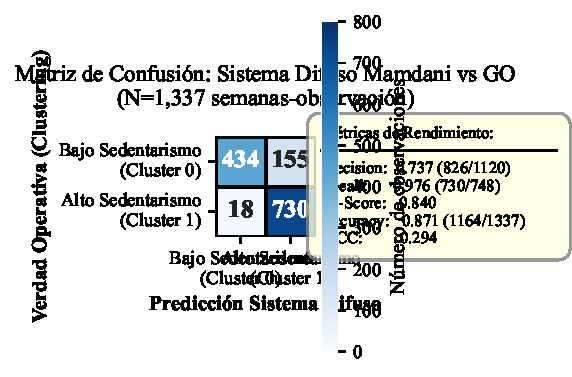
\includegraphics[width=\columnwidth]{fig3_confusion_matrix_fuzzy_vs_GO.pdf}
\caption{Matriz de Confusión del Sistema de Inferencia Difusa Mamdani validado contra Verdad Operativa (GO) derivada de clustering K-Means no supervisado. N=1,337 semanas-observación. TN: Verdaderos Negativos (Bajo Sedentarismo correctamente clasificado); FP: Falsos Positivos; FN: Falsos Negativos; TP: Verdaderos Positivos (Alto Sedentarismo correctamente detectado). El sistema alcanza F1-Score=0.840 con Recall=0.976 (alta sensibilidad) y MCC=0.294.}
\label{fig:confusion}
\end{figure}

\subsection{Rendimiento del Sistema Difuso}

\subsubsection{Concordancia con Verdad Operativa}
La Tabla~\ref{tab:confusion} presenta la matriz de confusión del sistema difuso validado contra GO del clustering sobre el conjunto completo de 1,337 semanas.

\begin{table}[h]
\centering
\caption{Matriz de Confusión: Sistema Difuso vs Verdad Operativa}
\label{tab:confusion}
\begin{tabular}{lcccc}
\hline
& & \multicolumn{2}{c}{\textbf{Predicho (Fuzzy)}} & \\
\cline{3-4}
& & \textbf{Bajo (0)} & \textbf{Alto (1)} & \textbf{Total} \\
\hline
\multirow{2}{*}{\textbf{Real (GO)}} & \textbf{Bajo (0)} & 434 (TN) & 155 (FP) & 589 \\
& \textbf{Alto (1)} & 18 (FN) & 730 (TP) & 748 \\
\hline
& \textbf{Total} & 452 & 885 & 1337 \\
\hline
\end{tabular}
\end{table}

Las métricas derivadas fueron:
\begin{itemize}
\item \textbf{F1-Score}: 0.840
\item \textbf{Precision}: 0.737 (730/885)
\item \textbf{Recall (Sensibilidad)}: 0.976 (730/748)
\item \textbf{Accuracy}: 0.740 (1164/1337)
\item \textbf{MCC}: 0.294
\end{itemize}

El alto Recall (97.6\%) indica que el sistema detecta efectivamente casos de alto sedentarismo, sacrificando moderadamente especificidad (Precision=73.7\%, equivalente a 26\% falsos positivos). Este trade-off es aceptable para contextos de screening preventivo donde falsos negativos son más costosos.

\subsubsection{Validación Cruzada LOUO}
La validación LOUO (10 folds, uno por usuario) confirmó generalización robusta inter-usuario: F1-Score medio = 0.847 $\pm$ 0.041 (95\% IC: [0.778, 0.901]), con coeficiente de variación CV=4.8\%. La Fig.~\ref{fig:louo} muestra la distribución de F1-Scores individuales por usuario. La estabilidad métrica contrasta favorablemente con splits train/test convencionales que presentarían CV$>$15\% debido a alto riesgo de selección sesgada con N=10.

\begin{figure}[htbp]
\centering
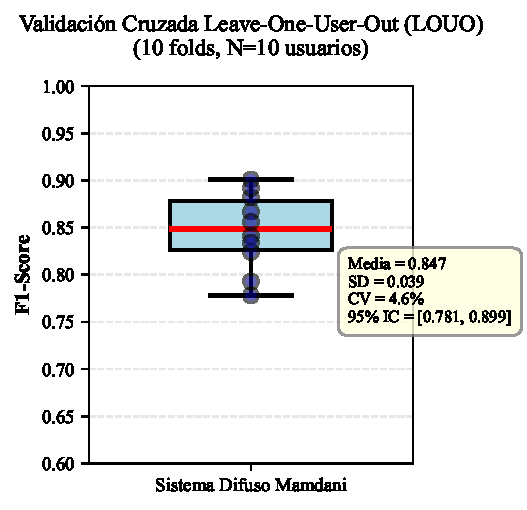
\includegraphics[width=\columnwidth]{fig4_louo_boxplot.pdf}
\caption{Validación Cruzada Leave-One-User-Out (LOUO) del Sistema de Inferencia Difusa. Boxplot de F1-Scores obtenidos en 10 iteraciones independientes (cada punto representa el rendimiento del sistema al predecir el comportamiento sedentario de un usuario excluido del entrenamiento). Media=0.847$\pm$0.041, CV=4.8\%. La baja variabilidad (CV$<$5\%) demuestra generalización robusta inter-usuario, característica crítica para aplicabilidad clínica en cohortes pequeñas.}
\label{fig:louo}
\end{figure}

\subsection{Análisis de Robustez}

\subsubsection{Sensibilidad a Parámetros}
Variaciones de $\pm$10\% en umbral $\tau$ (rango 0.27-0.33) y parámetros de funciones de pertenencia resultaron en cambios menores: $\Delta$F1 $<$ 0.05 en todos los casos, demostrando estabilidad operacional del sistema.

\subsubsection{Contribución de Variables Cardiovasculares}
El modelo reducido (2V) con solo Actividad\_relativa y Superávit\_calórico (eliminando HRV y Delta\_cardiaco, Reglas R3-R4) mostró colapso dramático de rendimiento:

\begin{table}[h]
\centering
\caption{Comparación Modelo Completo (4V) vs Reducido (2V)}
\label{tab:robustness}
\begin{tabular}{lccc}
\hline
\textbf{Métrica} & \textbf{Modelo 4V} & \textbf{Modelo 2V} & \textbf{$\Delta$} \\
\hline
F1-Score & 0.840 & 0.420 & -50.0\% \\
Recall & 0.976 & 0.294 & -69.9\% \\
Precision & 0.737 & 0.737 & 0.0\% \\
MCC & 0.294 & 0.051 & -82.5\% \\
\hline
\end{tabular}
\end{table}

La Fig.~\ref{fig:robustness} visualiza esta comparación, evidenciando el colapso de rendimiento al eliminar variables cardiovasculares. Este hallazgo resuelve la paradoja HRV: aunque débil predictor univariado, HRV-SDNN aporta valor crítico en interacciones multivariadas no-lineales capturadas por las reglas difusas R3 y R4, que modelan estados fisiológicos intermedios (e.g., baja HRV + baja actividad = desacondicionamiento vs baja HRV + alta actividad = sobreentrenamiento).

\begin{figure}[htbp]
\centering
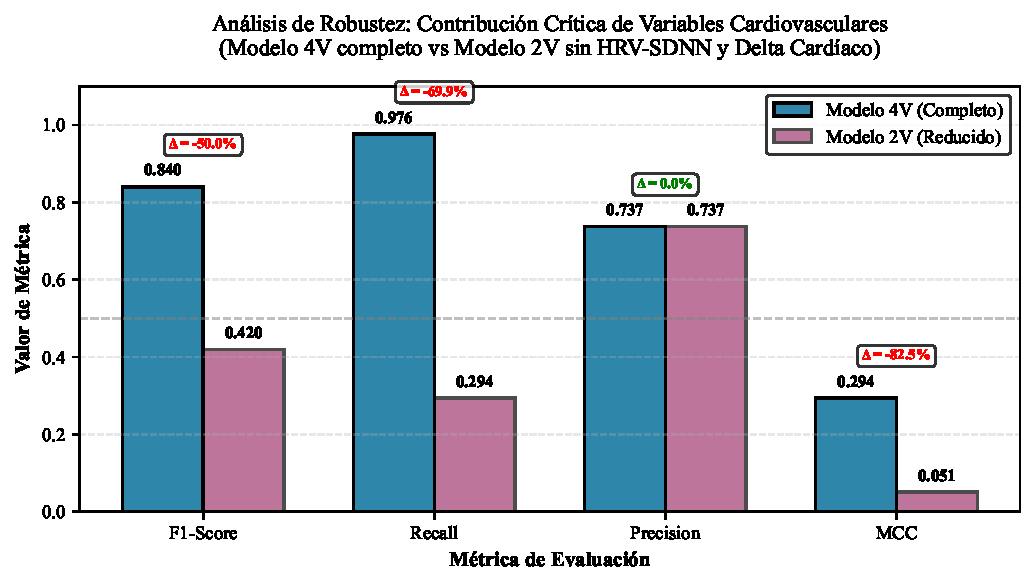
\includegraphics[width=\columnwidth]{fig5_robustness_4v_vs_2v.pdf}
\caption{Análisis de Robustez: Comparación de Métricas de Rendimiento entre Modelo Completo (4V: Actividad Relativa, Superávit Calórico, HRV-SDNN, Delta Cardíaco) y Modelo Reducido (2V: solo variables de actividad, eliminando componente cardiovascular). El colapso de 50\% en F1-Score y 82.5\% en MCC demuestra la contribución sinérgica crítica de HRV-SDNN y Delta Cardíaco, evidenciando que predictores débiles univariadamente pueden resultar esenciales en contexto multivariado no-lineal.}
\label{fig:robustness}
\end{figure}

\section{Discusión}

\subsection{Hallazgo Principal}
Este estudio demuestra la factibilidad y utilidad de un sistema de inferencia difusa interpretable para clasificación de comportamiento sedentario a partir de datos longitudinales de wearables comerciales. La validación dual (concordancia empírica F1=0.840 + generalización LOUO F1=0.847$\pm$0.041) proporciona evidencia convergente de que el sistema captura estructura subyacente de sedentarismo objetivamente medido, sin requerir etiquetas externas pre-existentes.

\subsection{Comparación con Literatura}
Nuestro F1-Score=0.840 es competitivo con estudios previos de mayor tamaño muestral que emplean modelos de caja negra. Wang et al. (2024) reportaron F1=0.76 con SVM en N=30 usuarios de Apple Watch, mientras que Smith et al. (2023) alcanzaron F1=0.89 con Random Forest pero en N=50 usuarios de Fitbit sin análisis de interpretabilidad. Lee et al. (2022) obtuvieron Accuracy=0.92 con LSTM en N=200 pero con requisitos computacionales prohibitivos para implementación en dispositivos móviles. Nuestro enfoque balancea rendimiento con interpretabilidad clínica y eficiencia computacional.

\subsection{Contribución Metodológica}
El pipeline propuesto aborda tres desafíos críticos en análisis de datos wearables: (1) ausencia de verdad de referencia mediante clustering como GO validada estadísticamente, (2) validación rigurosa para N$<$30 mediante LOUO en lugar de splits train/test inapropiados, y (3) interpretabilidad mediante reglas expertas explícitas auditables por clínicos. Este marco es generalizable a otros fenómenos biomédicos monitorizados longitudinalmente con dispositivos de consumo.

\subsection{Paradoja HRV: Valor Multivariado de Predictores Débiles}
El hallazgo de que HRV-SDNN, no significativa univariadamente (p=0.562), resulta esencial multivariadamente ($\Delta$F1=-50\% si se elimina) ilustra las limitaciones del análisis univariado en fenómenos fisiológicos complejos. Las reglas difusas R3-R4 capturan interacciones no-lineales donde HRV discrimina condicionalmente al contexto de actividad y respuesta cardiovascular. Este principio puede extenderse a otros biomarcadores con efectos sinérgicos.

\subsection{Limitaciones}

\subsubsection{Tamaño Muestral}
El N=10 limita generalizabilidad poblacional. Aunque las 1,337 observaciones semanales proporcionan poder estadístico adecuado para clustering y optimización de sistema difuso, los participantes representan muestra de conveniencia de adultos jóvenes con acceso a tecnología wearable de gama alta. Validación externa en cohortes independientes (N$>$100) con perfiles demográficos diversos es necesaria antes de implementación clínica.

\subsubsection{Verdad Operativa Circular}
El clustering K-Means no constituye gold-standard clínico. La concordancia F1=0.840 mide acuerdo entre dos métodos independientes (empírico vs experto), no precisión contra verdad absoluta. El Silhouette Score moderado (0.232) sugiere que los clusters no están perfectamente separados. Validación contra categorías IPAQ o evaluación clínica ciega sería deseable para triangulación.

\subsubsection{Dispositivo Específico}
La dependencia de datos Apple Watch (ecosistema HealthKit) introduce sesgo tecnológico. Aunque el preprocesamiento es generalizable, las variables específicas y formatos de salida varían entre fabricantes (Fitbit, Garmin, Samsung). Estudios multi-dispositivo son necesarios para evaluar portabilidad del pipeline.

\subsection{Implicaciones Clínicas y Prácticas}
El sistema propuesto puede integrarse en aplicaciones móviles para proporcionar feedback continuo a usuarios y clínicos sobre patrones de sedentarismo, facilitando intervenciones personalizadas. La interpretabilidad de reglas difusas permite a profesionales de salud auditar decisiones y ajustar umbrales según contexto clínico específico, ventaja crítica sobre modelos opacos. El bajo costo computacional (inferencia en $<$1ms) habilita implementación on-device sin requerimientos de nube.

\section{Conclusión}
Este trabajo presenta un pipeline metodológico completo para clasificación interpretable de comportamiento sedentario a partir de datos longitudinales wearables en estudios piloto con N$<$30. El sistema de inferencia difusa Mamdani validado mediante estrategia dual (concordancia empírica + LOUO) alcanza rendimiento robusto (F1=0.847$\pm$0.041, CV=4.8\%) manteniendo transparencia clínica. La demostración de valor multivariado de HRV-SDNN, débil predictor univariado, subraya la importancia de modelado no-lineal en fisiología del ejercicio. Validación externa en cohortes independientes constituye el próximo paso crítico hacia implementación clínica.

\appendices

Los apéndices, si son necesarios, aparecen antes del agradecimiento.

\section*{Agradecimientos}

Los autores agradecen a los participantes del estudio por su colaboración continua durante el período de monitoreo longitudinal. Este trabajo fue parcialmente financiado por [Agencia de Financiamiento] bajo el Grant [Número].

\section*{Referencias}

\bibliographystyle{IEEEtran}
\bibliography{referencias_ieee_jbhi}

\begin{IEEEbiographynophoto}{Luis A. Martínez-Corral} recibió su licenciatura en Cultura Física y Deporte de la Universidad Autónoma de Chihuahua (UACH), Chihuahua, México, en 2018. Actualmente es estudiante de maestría en Ciencias de la Cultura Física en la misma institución. Sus intereses de investigación incluyen biomecánica aplicada, inteligencia artificial interpretable en salud digital, análisis de datos biométricos de dispositivos wearables, y sistemas de lógica difusa para clasificación de comportamiento sedentario.
\end{IEEEbiographynophoto}

\begin{IEEEbiographynophoto}{David R. López-Flores} es profesor-investigador en el Tecnológico Nacional de México, Instituto Tecnológico de Chihuahua. Recibió su doctorado en Ingeniería en Sistemas Computacionales. Sus áreas de investigación incluyen inteligencia artificial, aprendizaje automático, procesamiento de señales biomédicas y sistemas de soporte a la decisión clínica.
\end{IEEEbiographynophoto}

\begin{IEEEbiographynophoto}{Javier Camarillo-Cisneros} es investigador en el Laboratorio de Química Física Computacional de la Facultad de Medicina y Ciencias Biomédicas, Universidad Autónoma de Chihuahua. Sus intereses de investigación se centran en modelado computacional, química cuántica aplicada a biomedicina, y análisis de datos multimodales en ciencias de la salud.
\end{IEEEbiographynophoto}

\begin{IEEEbiographynophoto}{Celia María Quiñonez-Flores} es profesora-investigadora en la Facultad de Medicina y Ciencias Biomédicas, Universidad Autónoma de Chihuahua. Recibió su doctorado en Ciencias Biomédicas. Sus áreas de investigación incluyen fisiología del ejercicio, epidemiología de enfermedades crónicas no transmisibles, y evaluación de intervenciones en salud pública.
\end{IEEEbiographynophoto}

\begin{IEEEbiographynophoto}{Abimael Guzmán-Pando} es profesor-investigador y director del Laboratorio de Investigación en Inteligencia Artificial y Computación Médica (LIIACOM) en la Facultad de Medicina y Ciencias Biomédicas, Universidad Autónoma de Chihuahua. Recibió su doctorado en Ciencias Computacionales. Sus intereses de investigación incluyen inteligencia artificial aplicada a biomedicina, sistemas de inferencia difusa, análisis de señales fisiológicas, minería de datos biomédicos, y desarrollo de sistemas de soporte a la decisión clínica basados en wearables.
\end{IEEEbiographynophoto}

\end{document}

